\documentclass[a4paper,11pt]{article}
\usepackage{inet-primitives}

\title{Spaghetti-nets : examples with primitive interaction nets}
\author{Eng Boris}
\date{}

\begin{document}
\maketitle

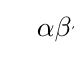
\begin{tikzpicture}
    \node (dummy) {};

    \inetcell[uphead, left=5mm of dummy]{c1}{$\alpha$}
    \inetcell[righthead, above=5mm of dummy]{c2}{$\beta$}
    \inetcell[downhead, right=5mm of dummy]{c3}{$\gamma$}
    \inetcell[lefthead, below=5mm of dummy]{c4}{$\omega$}
\end{tikzpicture}


\end{document}
